%%% LaTeX template file for UP poster.
%%% ------------------------------------------------------------------------------------------------

\documentclass[pageborders=False, colorscheme1, a0paper, 50pt]{upposter}
% Drawing page borders is useful when the poster will be printed
% on a larger paper size, and needs to be cut afterwards.
% In other cases it is best to omit option pageborders.

% \usepackage[ngerman]{babel} % german (hyphenation... )
\usepackage[english]{babel} % english (hyphenation... )
\usepackage[utf8]{inputenc}
\pdfcompresslevel=0

% TODO
\title{Hardware-Accelerated Load Balancing on Bluefield-3 DPUs - XenoFlow Implementation and Performance Evaluation}
%%% List the authors here.
% TODO
%\author{M. Itarbeiter}
%%% List the cooperations and funding partners here.
% TODO
\institute{\begin{tabular}{ll}
\Large Operating Systems and Distributed Systems \\
\Large Max Schrötter, Sten Heimbrodt, Bettina Schnor \\
\Large University of Potsdam
\end{tabular}}

% Block Style without borders
\defineblockstyle{Plain}{
	titlewidthscale=1,
	bodywidthscale=1
}{
	\setlength{\blocklinewidth}{0pt}
}


\begin{document}
	%%% Uncomment this to add the mathpluslogo
	% TODO 
	
	%%% This command creates your title.
	\maketitle % Create title

	
	
	
	%%% Here you can put your poster content.
	%%%
	%%% A box with a title is created by the following command:
	%%% \block{Title}{Content}
	%%% For a box without a titlebar just leave the title empty:
	%%% \block{}{Content}
	%%%
	%%% The content of a block allows regular latex code (with some exceptions).
	%%%
	%%% Blocks can span the width of the poster or can be placed inside columns.
	%%% Columns are defined like this:
	%%%
	%%% \begin{columns}
	%%% \column{.3} % this is a column spanning 30 percent of the width of the poster.
	%%% \block{Title1}{Content1}
	%%% \block{Title2}{Content2}
	%%% \column{.7} % this is a column spanning 70 percent of the width of the poster.
	%%% \block{Title3}{Content3}
	%%% \end{columns}
	%%%
	%%% At the very end of the poster creating process you should make sure that your
	%%% blocks at the end of the poster align. You can for example play around with
	%%% \vspace{2cm}
	%%%
	%%% Assuming your file is named 'poster.tex' you can compile it by opening a commandline,
	%%% navigating to the folder containing the file and typing
	%%%    pdflatex poster.tex
	%%%
	%%% A word to the papersize:
	%%% The frames at ZIB have b1paper format. Since the fontsizes and measurements should be uniform,
	%%% please use the following doumentclass and don't change neither the colorscheme nor
	%%% the fontsizes or fontfamilies:
	%%% \documentclass[grey,b1paper,fontserif]{zibposter}
	%%%
	%%% If you or your conference prefer a0paper or you like a different colorscheme
	%%% you can change these parameters in the documentclass.
	
	%%% --- begin content ------------------------------------------------------------------------------
%	\begin{columns}
%		
%		\column{0.55}
%		
\useblockstyle{Plain}
%\block{}{
	
%}

	
%		
%	\end{columns}
%	

\useblockstyle{upposter}
\block{Motivation}{
	The goal was to accelerate load balancing on Bluefield-3 DPUs by using hardware acceleration.
	This would allow for more efficient resource utilization and improved performance in data center and high performance computing environments. 
	The main challenge was to implement and evaluate the performance of XenoFlow, a software framework for hardware-accelerated load balancing for UDP traffic. 
	XenoFlow began as a research project and is beeing extended to support more features and use cases.
	%\begin{minipage}[t]{.3\linewidth}
		%\begin{itemize}
		%	\item Point 1
		%	\item Point 2
		%	\item Point 3
		%	\item ...
		%	\item Point 41
		%	\item Point 42
		%	\item Point 43
		%\end{itemize}
	%\end{minipage}
}

	
	\begin{columns}
		
		\column{.55}
		
		\block{XenoFlow}{
			XenoFlow is a software framework for hardware-accelerated load balancing for UDP traffic:
			\begin{itemize}
				\item It is designed to run on Bluefield-3 DPUs, which are specialized processors for data center and high performance computing environments.
				\item Currently, XenoFlow supports basic L3 load balancing features for UDP traffic.
				\item The framework is implemented in C and uses the DOCA Flow API to interact with the hardware acceleration features of the Bluefield-3 DPUs.
			\end{itemize}
		}
		
		\block{Bluefield Architecture}{
			\begin{tikzfigure}
				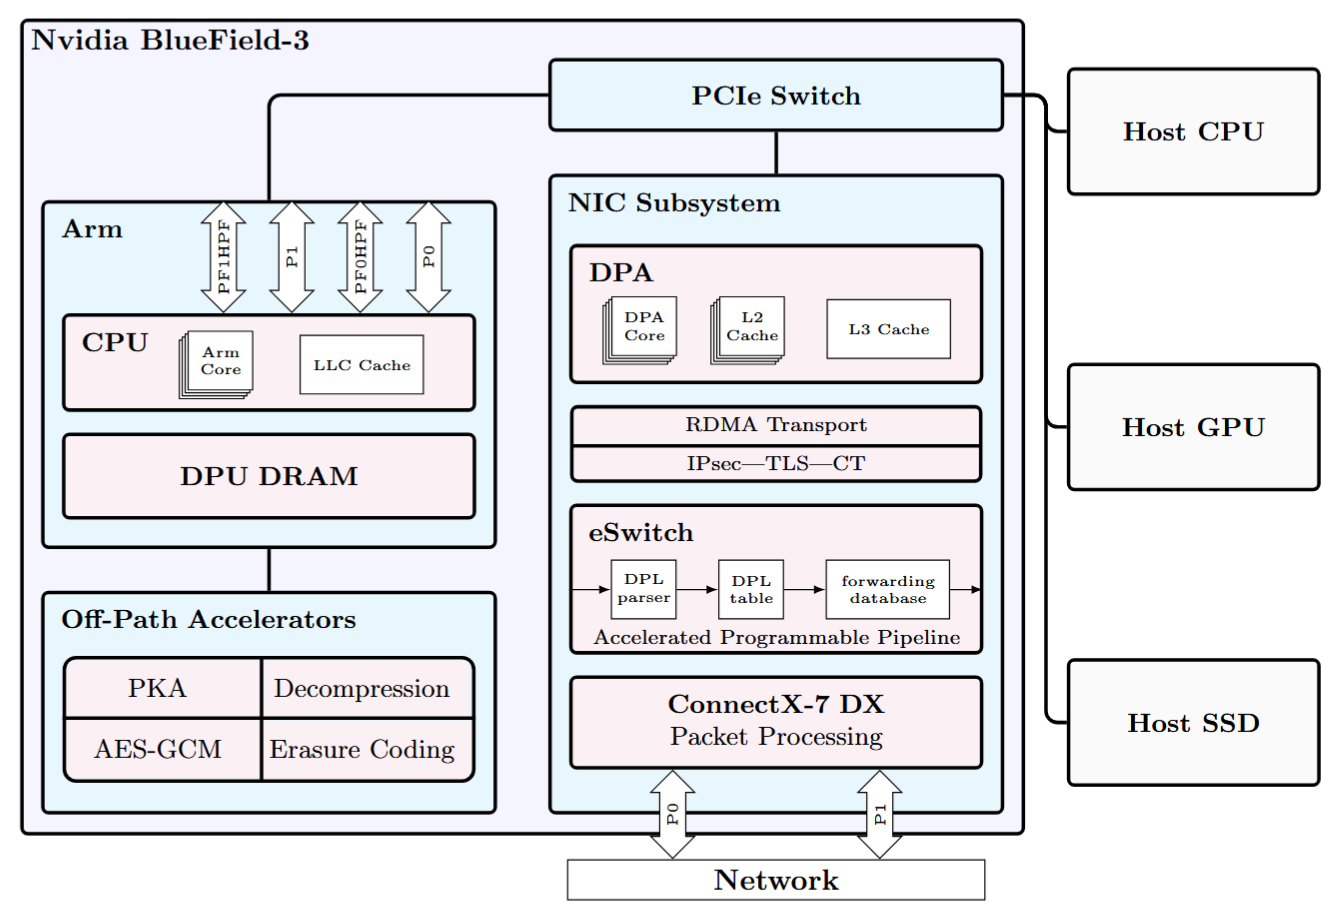
\includegraphics[width=1\linewidth]{graphics/bluefield.png}
			\end{tikzfigure}

			\vspace*{0mm}
		}

		\block{DOCA Flow API}{
			\begin{itemize}
				\item NVIDIA provided header files and compiled shared libraries, which are used to interact with the hardware acceleration features.
				\item Flows consist of \textbf{pipes}, which are sequences of actions that can be executed on the hardware.
				\item Pipes contain \textbf{entries}, which define specific actions to be performed on packets that match certain criteria.
				\item Flow allows for matching on various L3 and L4 header fields aswell as actions such as forwarding, dropping, and modifying packet headers.
			\end{itemize}
		}
        \block{Publications}{
			\begin{thebibliography}{9}
				\bibitem{ref1} M. Schrötter, S. Heimbrodt, B. Schnor. XenoFlow: How Fast Can a SmartNIC-Based DNS Load Balancer Run?
				\textit{GI/ITG International Conference on Architecture of Computing Systems (ARCS)} 2026.    
                \bibitem{ref2} S. Heimbrodt, Implementierung und Evaluation eines hardwarebeschleunigten Load-Balancers auf einer Nvidia Bluefield DPU Architektur
                \textit{Bachelorarbeit, Universität Potsdam}, 2025.
			\end{thebibliography}

			\vspace{0mm}
		}
		
		\column{.45}
		
		\block{Flow Pipe}{
			\begin{tikzfigure}
				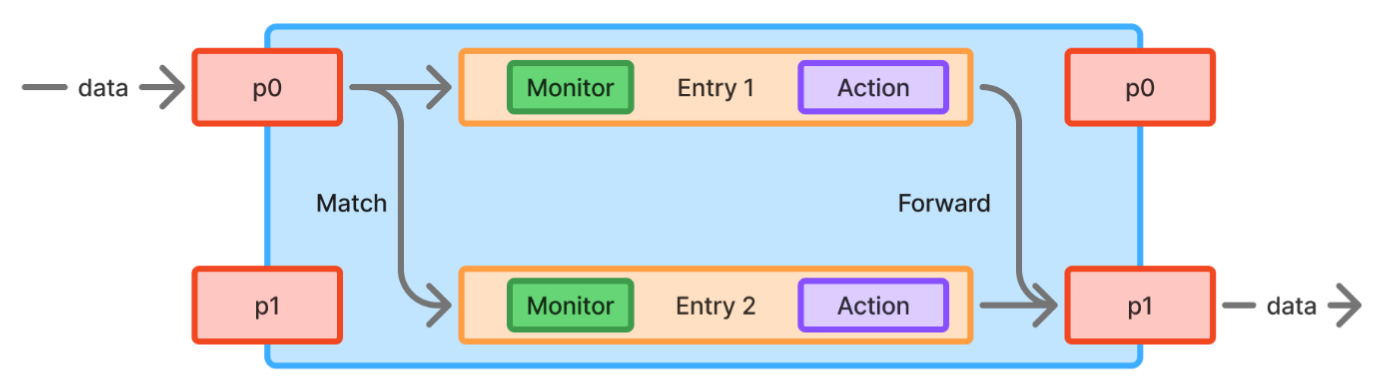
\includegraphics[width=1\linewidth]{graphics/pipe.png}
			\end{tikzfigure}
		}
		
		\block{Performance}{
			\begin{tikzfigure}
				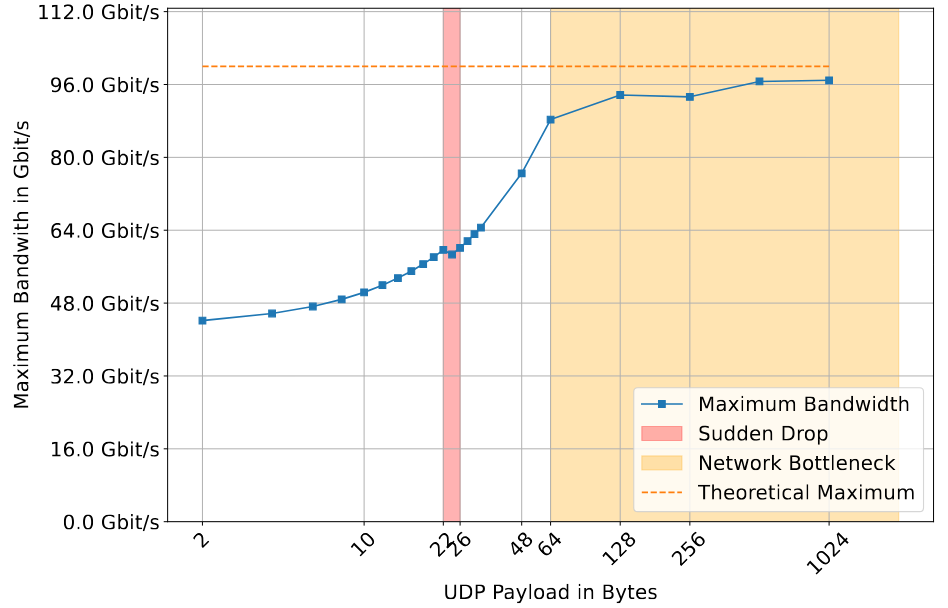
\includegraphics[width=1\linewidth]{graphics/Screenshot 2026-03-07 at 12-34-33 XenoFlow How Fast Can a SmartNIC-Based DNS Load Balancer Run - 2509.21656v1.pdf.png}
				%\vspace*{0mm}
			\end{tikzfigure}
            \begin{tikzfigure}
                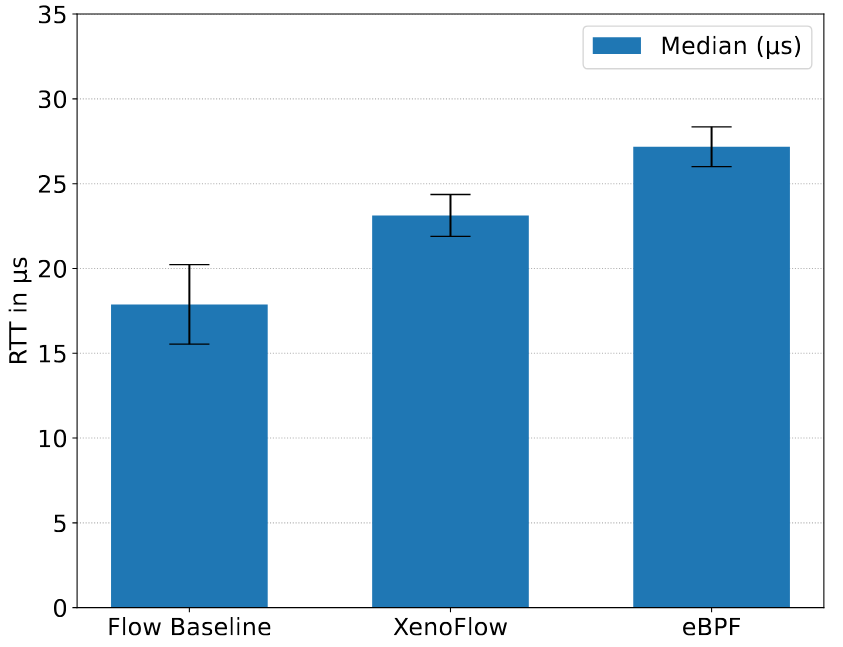
\includegraphics[width=0.8\linewidth]{graphics/Screenshot 2026-03-07 at 12-31-47 XenoFlow How Fast Can a SmartNIC-Based DNS Load Balancer Run - 2509.21656v1.pdf.png}
            \end{tikzfigure}
		}
		
		\block{Current Goals}{
			\begin{itemize}
			    \item Extending configuration via 
			\end{itemize}
		}
		
	\end{columns}
	
	\begin{columns}
		
		\column{.55}
		
		
		
		\column{.45}
		
		
		
	\end{columns}
	
	%%% --- end content --------------------------------------------------------------------------------
\end{document}
